\documentclass{article}
\usepackage[utf8]{inputenc}
\usepackage[T1]{fontenc}
\usepackage{microtype}
\usepackage{graphicx}
\usepackage{booktabs}
\usepackage{amsmath,amssymb,amsthm}
\usepackage{array}
\usepackage{placeins}
\usepackage{url}
\usepackage[hyperfootnotes=false]{hyperref}
\usepackage[preprint]{icml2026}
\hypersetup{pdftitle={From Typed Language Structure to Bayesian Learner Decisions},pdfauthor={Anonymous Authors},pdfsubject={Nabu 1.15.0 implementation and synthetic verification; no human efficacy claim},colorlinks=true,urlcolor=blue,citecolor=blue,linkcolor=blue}
\icmltitlerunning{Auditable Bayesian Learner Decisions}
\icmlkeywords{hierarchical Bayes, language learning, value of information, provenance}
\newtheorem{proposition}{Proposition}
\newcommand{\Nabu}{\textsc{Nabu}}
\newcommand{\E}{\mathbb{E}}
\newcommand{\sig}{\operatorname{sigmoid}}
\newcommand{\artifact}[1]{\nolinkurl{#1}}
% Generated from docs/learner-evaluation/results.json and verification logs.
\newcommand{\LearnerTasks}{93}
\newcommand{\LearnerLanguages}{12}
\newcommand{\LearnerContrasts}{8}
\newcommand{\LearnerExactCases}{8}
\newcommand{\LearnerStructuralCases}{5}
\newcommand{\LearnerArabicPrior}{0.504}
\newcommand{\LearnerArabicPosterior}{0.789}
\newcommand{\LearnerSpanishBorrowed}{0.525}
\newcommand{\LearnerSpanishCounter}{0.358}
\newcommand{\LearnerUntestedForm}{0.220}
\newcommand{\LearnerReferenceMean}{0.70578}
\newcommand{\LearnerSampledMean}{0.69779}
\newcommand{\LearnerReferenceError}{0.00799}
\newcommand{\LearnerBrierPrior}{0.2465}
\newcommand{\LearnerBrierPosterior}{0.0897}
\newcommand{\LearnerLogPrior}{0.6862}
\newcommand{\LearnerLogPosterior}{0.3402}
\newcommand{\LearnerRuntime}{805.8}
\newcommand{\LearnerNodeTests}{855}
\newcommand{\LearnerDOMTests}{72}
\newcommand{\LearnerAPITests}{483}

\makeatletter
\renewcommand{\printAffiliationsAndNotice}[1]{%
 \global\icml@noticeprintedtrue%
 {\let\thefootnote\relax\footnotetext{\hspace*{-\footnotesep}%
 Anonymous research and software draft, November 2026. Not submitted or peer
 reviewed. Results concern executable contracts and synthetic cases, not human
 learning efficacy.}}}
\makeatother
\begin{document}
\twocolumn[
\icmltitle{From Typed Language Structure to Bayesian Learner Decisions:\texorpdfstring{\\}{ }
Auditable Hierarchies in Nabu}
\begin{icmlauthorlist}
\textbf{Anonymous Authors}
\end{icmlauthorlist}
\vskip 0.3in
]
\printAffiliationsAndNotice{}

\begin{abstract}
Typed linguistic relations can preserve the ingredients of a language task
without identifying what a learner knows or which intervention is useful.
We implement the missing inferential and decision layers in an existing
multilingual reader. A versioned observation bridge admits only scoped,
auditable first responses under declared task conditions. A crossed Bayesian
model separates language, response mode, lexical base, morphological pattern,
explicitly shared meaning, context, and whole-form memory; variance
hyperparameters govern partial pooling. Its likelihood combines required
components with an optional memory route, guessing, lapses, and observational
time and practice terms. Bounded elliptical slice and variance-Gibbs sampling
runs locally, with cancellation, diagnostics, and a distinct posterior
namespace. A one-step decision rule compares immediate task failure and effort,
and recommends a diagnostic only when its expected downstream decision value
pays for its cost. The release includes \LearnerTasks{} new authored tasks in
\LearnerLanguages{} languages and explicit mappings for \LearnerContrasts{}
existing contrasts. Numerical reference checks, synthetic decision cases,
provenance tests, and executable application tests examine the implemented
contracts. This establishes a working, inspectable statistical architecture;
it does not establish measurement validity, causal language transfer, or
improved human learning.
\end{abstract}

\section{Problem and Contribution}

A successful response to Arabic \emph{maktub} (written) is compatible with
several explanations. A learner may retrieve a stored word, combine a lexical
base with a familiar form pattern, use a recently supplied cue, or guess.
Conversely, an unsuccessful response need not isolate one missing ingredient.
An English or Spanish expression with a related meaning creates a further
question: which part of the response could reasonably share evidence across
languages?

An implementation must answer these questions at different levels. Linguistic
structure declares which relations and analyses are available. Observations
record what was displayed, supplied, or answered. A statistical model assigns
likelihoods to those observations. A decision model describes what an action
would provide and what the learner values. Collapsing these levels makes
graph connectivity look like competence, or uncertainty reduction look like
learning benefit.

The preceding \Nabu{} release supplied a typed incidence graph, source-qualified
witnesses, an immutable observation ledger, and deterministic support rules.
It deliberately left overall competence unknown. The present release adds a
live Bayesian learner model and a decision interface while retaining that
ledger. The contributions are an integrated, executable contract:

\begin{enumerate}
\item a versioned bridge from exact task observations to a crossed,
conjunctive learner likelihood;
\item local approximate posterior inference with learned pooling scales,
explicit cross-language mappings, and separate response modes;
\item a decision-relevant value-of-information calculation with actual
support actions, time budgets, and a functional Continue action; and
\item reproducible numerical and integration checks that expose the boundary
between implemented inference and empirical educational claims.
\end{enumerate}

The statistical ingredients are established. The contribution is their
auditable integration in a working language application, together with
failure cases that distinguish structurally valid representations from
statistically or causally justified conclusions.

\section{Foundations and Observation Contract}

\paragraph{Related mathematical ideas.}
Conjunctive cognitive assessment models express the need for several
components in one response \citep{junker2001cognitive}. Hierarchical Bayesian
domain adaptation provides a useful precedent for sharing information while
retaining domain-specific parameters \citep{finkel2009hierarchical}.
Knowledge tracing addresses hidden learner state
\citep{corbett1994knowledge}, while trainable repetition models explicitly
represent recall over time \citep{settles2016trainable}. None of these
connections establishes the validity of the present linguistic labels.
We use them as modeling foundations, with separate numerical and application
verification.

\paragraph{Three persistent identities.}
An event has an immutable event ID, an episode and attempt identity, and an
exact task/source reference. The reference retains the task version,
occurrence, reading, input and output modalities, scorer, rubric, analysis
version, assistance flags, and account/team actor. A displayed word, a lookup,
a skip, an authored correct response, and a posterior prediction remain
different records. The original ledger continues to report
\texttt{competence: null}; inferred probabilities live in a separate object.

The bridge resolves the exact recorded task and scoring references. Unknown,
changed, quarantined, future, ambiguous, duplicated, or unsupported records
cannot silently enter the response likelihood. Only an unambiguous first
response for an eligible task episode is admitted. Assisted responses remain
auditable but normally do not update unaided performance. A deliberately
conditioned task is an explicit exception: when the base meaning is supplied,
an approved pattern task may inform only its remaining mapped components.
It earns no unaided credit for that base.

The live interface covers the source during a check, freezes the first
submitted payload across storage retries, and records feedback separately.
Reopening within a bounded session reconstructs prior help. An immediate
answer repetition therefore cannot become a new independent trial by closing
the dialog. Actor or team changes cancel pending inference and clear the
visible posterior. These are operational controls, not proofs of psychological
independence: unrecorded help and dependence between different questions remain
possible.

\paragraph{Declared task map.}
Let task \(q\) specify language \(\ell_q\), mode \(m_q\), word identity \(w_q\),
context \(x_q\), a required component set \(C_q\), and an optional whole-form
memory route. Each component has an ID, a kind (meaning, lexical base, or
pattern), and an optional, explicit transfer-group ID. A matching string or
graph path does not create such a group. Task versions and analysis
fingerprints make the declaration inspectable.

The authored slice includes contrasting Arabic base recall, conditioned
pattern application, full-form recall, and contextual meaning checks. English
and Spanish lexical exceptions retain an item-memory route without joining a
universal irregular-word rule. A small vocabulary slice spans twelve
languages. Its production tasks require local lexical forms; its recognition
tasks require a local form and a declared meaning. A shared concept therefore
cannot by itself satisfy an unknown foreign form. Recognition and production
have distinct parameters; recognizing a base does not count as recalling it.

\section{Crossed Hierarchical Learner Model}
\label{sec:model}

\subsection{Effects and Partial Pooling}

For learner \(u\), language \(\ell\), mode \(m\), component \(c\), word \(w\),
and context \(x\), the default component logit is
\begin{equation}
\begin{split}
\eta_{u q c}(t)={}&\mu_{\ell m}+a_{u\ell m}
 +b_{u\ell c m}+v_{u\ell w m}+z_{u\ell x m}\\
 &+\mathbf{1}_{g(c)\ne\varnothing}s_{u g(c)m}
 +D_{u\ell m}(t;c)-d_q .
\end{split}
\label{eq:eta}
\end{equation}
Here \(g(c)\) is the pair (component kind, declared transfer-group ID), or
\(\varnothing\) when no sharing is declared. Absent context terms are zero.
Each named effect has a zero-centered
Gaussian prior whose variance is shared by its kind and response mode.
For variance group \(k\),
\begin{equation}
 \theta_j\mid \tau_k^2\sim\mathcal N(0,\tau_k^2),\qquad
 \tau_k^2\sim\operatorname{IG}(\alpha_k,\beta_k).
\label{eq:hierarchy}
\end{equation}
The default \(\alpha_k=3\) and
\(\beta_k=(\alpha_k-1)s_k^2\) make the prior mean of the variance \(s_k^2\).
The scales are explicit initial assumptions in the code. They are neither
population estimates nor noninformative limits. Variance priors can materially
affect sparse hierarchical inference \citep{gelman2006prior}; the export
therefore records both prior settings and the sampled hyperparameters.

Repeated evidence for one pattern updates the shared pattern variable and
the posterior over its pooling variance. Word, root, language, and context
effects allow systematic departures. Sparse tasks receive information through
these variables; direct evidence can distinguish their local effects.
This is partial pooling through a joint posterior, not a fixed weighted
average of neighboring correctness counts.

The shared term \(s_{ugm}\) is present only for a declared transfer group.
Language-specific component effects remain in the same response logit.
The model learns the relative variance of shared and local effects under that
factor structure. It does not learn an unrestricted signed covariance matrix,
infer equivalence from spelling, or discover a universal semantic ontology.
The induced sharing is a modeling hypothesis with uncertainty.

\paragraph{Authorized population layer.}
By default the fit uses only the current actor's accepted observations.
An explicit cohort API can add population-level means for the same named
effects and learner-specific deviations. It requires a named population
scope and explicit authorization flags. No live application action silently
reads other learners' private events. A separate reusable calibration helper
returns a moment-matched approximation to the cohort hyperposterior; the full
joint fit remains available for research. Neither form constitutes human
calibration without an appropriate dataset.

\subsection{Conjunction and a Whole-Form Alternative}

Let \(p_{uqc}(t)=\sig(\eta_{uqc}(t))\), and let
\(r_{uq}(t)\) be the whole-form memory probability when that route is enabled.
The memory logit has its own language-, mode-, and word-specific random
effect, an optional context effect, and the same form of temporal covariates.
The implemented success probability is
\begin{equation}
\begin{split}
 A_{uq}(t)&=\prod_{c\in C_q}p_{uqc}(t),\\
 I_{uq}(t)&=r_{uq}(t)+(1-r_{uq}(t))A_{uq}(t),\\
 \pi_{uq}(t)&=g_q+(1-g_q-s_q)I_{uq}(t),\\
 Y_{uq}(t)&\sim\operatorname{Bernoulli}(\pi_{uq}(t)).
\end{split}
\label{eq:likelihood}
\end{equation}
Here \(g_q\) is a guessing floor and \(s_q\) a lapse probability.
An empty component set is permitted only for a memory task; in that case
\(A_{uq}=0\), avoiding vacuous success. A disabled memory route has \(r_{uq}=0\).
The current tasks declare nuisance values rather than estimating them from
people: three-choice items use a \(1/3\) guessing floor, typed items use
\(0.01\), and the lapse rate is \(0.05\).

The conjunction encodes required ingredients within the modeled compositional
route. The whole-form alternative explains why success need not establish
every ingredient. Guessing and lapses further distinguish observed correctness
from a deterministic knowledge label. The product is an explicit
conditional-execution assumption; component response events have not been
separately observed merely because the complete answer was correct.

\begin{proposition}[One combined task does not identify its routes]
In the simplified model with known nuisance terms, fixed component
probabilities \(b,p\), and whole-form probability \(r\), repeated responses
to the same combined task identify at most
\(r+(1-r)bp\). They do not generally identify \(b,p,r\) separately.
\end{proposition}
\begin{proof}
The Bernoulli likelihood depends on the triple only through that scalar.
For \(r=0\), every pair with the same product \(bp\) has the same likelihood.
Allowing \(r\) adds further equivalent triples. A proper prior can produce
a proper posterior over them without making the likelihood one-to-one.
\end{proof}

Contrasts change the task map and may break this ambiguity. Base recall,
pattern application with the base supplied, and full-form recall have
different likelihoods. They do not automatically prove that a psychological
decomposition is correct. The engine reports component identification as
unestablished and flags components observed only together.

\subsection{Time and Practice}

For an accepted history of component opportunities, let \(n_c(t)\) be the
number of prior responses and \(\Delta_c(t)\) days since its most recent
accepted opportunity. The implemented association is
\begin{equation}
\begin{split}
 D_{u\ell m}(t;c)={}&
 \lambda_{u\ell m}\log(1+n_c(t))\\
 &-\kappa_{u\ell m}\log(1+\Delta_c(t)),
\end{split}
\label{eq:time}
\end{equation}
where \(\kappa_{u\ell m}=\operatorname{softplus}(-3+\phi_{u\ell m})\).
No prior opportunity gives zero lag and count. Memory has its own opportunity
history; a response in Arabic does not reset the last-practice time of a
Spanish lexical form. Histories are built in time order, excluding future
events and episode duplicates.

The practice coefficient is signed. The decay coefficient is nonnegative
under this chosen response model. Both have hierarchical priors and remain
prior-sensitive without varied repeated observations. This is an observational
response model. A practice-count coefficient does not identify the causal
effect of assigning practice, and its value is not used as a claimed learning
gain in the decision layer.

\section{Bounded Posterior Inference}

Conditional on the variances, the latent effect vector has a Gaussian prior.
The implementation uses elliptical slice sampling
\citep{murray2010elliptical} for this vector and a Gibbs update for each
variance group. Coefficients absent from the observed likelihood are
analytically marginalized during fitting. If \(A_k\) is the active set for
group \(k\), the update is
\begin{equation}
 \tau_k^2\mid\theta_A \sim
 \operatorname{IG}\left(
 \alpha_k+\frac{|A_k|}{2},
 \beta_k+\frac12\sum_{j\in A_k}\theta_j^2
 \right).
\label{eq:gibbs}
\end{equation}
Inactive coefficients are then drawn conditionally on the retained variances
when constructing each full posterior draw. The seeded implementation returns
aligned joint draws and normalized weights.
All response probabilities for a draw use the same latent vector. Preserving
that alignment is necessary for downstream decision reweighting.

The default engine runs two chains with 96 warm-up iterations and 64 retained
draws per chain. Default candidate and history limits are 128 tasks and 256
accepted observations; bounds are explicit and checked before or during
fitting. The asynchronous API yields periodically and supports cancellation.
The live interface performs one longer fit, with 384 warm-up iterations and
256 retained draws per chain, if its first predictive chain check fails.
It does not manufacture more evidence or alter observation weights when it
spends more computation.

Exports include chain diagnostics, effective sample estimates, caps reached,
omitted observation IDs, the task map, hyperparameters, and posterior draws.
The implemented diagnostics are lightweight predictive checks, not a
certificate of convergence of every latent parameter. The paper and UI use
the term approximate posterior accordingly. An unstable fit is displayed as
provisional; the decision layer suppresses extra diagnostics from a fit whose
convergence check explicitly fails. Numerical stability and model
identifiability are separate questions.

\section{Actions and Decision-Relevant Information}
\label{sec:decision}

Let \(T\) be selected target tasks with normalized weights \(\omega_q\).
Continue has zero added time and cost. A support action declares which
component it supplies, the exact affected tasks, its actual cue text, duration,
and effort cost. A diagnostic names a real available task. Unsupported
components, unavailable tasks, prohibited practice, and actions exceeding the
budget are excluded before comparison.

For a terminal action \(a\), a supplied component is set to one in the
conditional task calculation only for its declared affected targets.
The learner posterior is unchanged. If \(t_a\) is action duration and
\(c_a\) its explicit effort cost, posterior risk is
\begin{equation}
 R(a\mid D)=c_a+
 \sum_{q\in T}\omega_q
 \E_{\theta\mid D}[1-\pi_q^{\,a}(\theta,t+t_a)].
\label{eq:risk}
\end{equation}
The interface currently uses one chosen target and
\(c_a=0.002\,t_a\), with time in seconds; the API permits explicit costs and
multiple weighted targets. These units are authored utility assumptions.
The criterion concerns immediate aided completion, not durable learning.

For a binary diagnostic \(d\), the same joint posterior draws supply
its predictive probability and the future action risks. For outcome
\(y\in\{0,1\}\),
\begin{equation}
 w_j^{(y)}=
 \frac{w_j\,\pi_d(\theta_j)^y[1-\pi_d(\theta_j)]^{1-y}}
 {\sum_iw_i\,\pi_d(\theta_i)^y[1-\pi_d(\theta_i)]^{1-y}}.
\label{eq:reweight}
\end{equation}
This is Bayes reweighting of the existing draws. It does not write either
hypothetical response to the learner's ledger. The rollout is explicitly
information-only: wall-clock time advances to diagnostic completion, but
practice counts and last-opportunity histories stay fixed during the
comparison. It assigns no benefit to a hypothetical practice opportunity
or reset of a forgetting clock. An actual saved response and refit do update
the history, so the subsequent live choice can also reflect those newly
observed conditions. The preposterior comparison follows
the expected-value-of-sample-information principle
\citep{heath2018efficient}; our binary calculation enumerates outcomes and
does not use that paper's moment-matching estimator.

To isolate information from time and feasibility, let \(\mathcal A_d\)
be the terminal actions still feasible after the diagnostic, evaluated at
that same future time. Then
\begin{equation}
\begin{split}
 \operatorname{EVSI}(d)
 ={}&\min_{a\in\mathcal A_d}R_d(a\mid D)\\
 &-\sum_yP(y\mid D,d)
       \min_{a\in\mathcal A_d}R_d(a\mid D,y).
\end{split}
\label{eq:evsi}
\end{equation}
The complete diagnostic loss adds its effort cost to the expected downstream
minimum. Comparison against the best action \emph{now} also accounts for the
delay and loss of feasible actions. A diagnostic is recommended only when
outcomes can change the terminal choice and the net improvement is positive.
Ties favor fewer interruptions.

\begin{proposition}[Information without a changed action]
Under the same downstream time, feasible set, posterior, and loss,
\(\operatorname{EVSI}(d)\ge0\). If one terminal action minimizes risk for every
possible diagnostic outcome, EVSI is zero.
\end{proposition}
\begin{proof}
For any fixed action, expected conditional risk equals its preposterior risk
by total expectation. The expected minimum is no larger than the minimum
of these expectations. If the same action attains every conditional minimum,
the inequality is equality.
\end{proof}

Thus a check may reduce uncertainty while being worth no interruption.
A diagnostic may also have positive EVSI but negative net value after its
time cost. The implementation exports both quantities and both outcome
branches. Continue remains available even when the posterior or action set
is unusable.

% Evaluation and appendices are maintained separately so generated results
% can be checked without editing the model definition.
\section{Executable Evaluation}
\label{sec:evaluation}

We evaluate numerical correctness, declared model behavior, and application
contracts separately. All learner outcomes in the numerical report are
synthetic. None were loaded into the live interface as user history.
The canonical record is
\artifact{docs/learner-evaluation/results.json}; its Markdown companion,
figures, and this paper's numerical macros are generated from the same file.
The default experiment seed is 140015. Fits use two chains, 384 warm-up
iterations, and 256 retained draws per chain unless the reference experiment
specifies otherwise.

\subsection{Independent Numerical Reference}

A one-dimensional submodel removes unrelated effects and dynamics, sets
the memory-logit prior to standard normal, and supplies eight successes and
two failures. Composite Simpson integration on a bounded logit interval
provides an independent reference for the response probability posterior.
This is a useful test because it evaluates a known density by a different
numerical method, rather than checking the sampler against its own update
equations.

The numerical reference mean is \LearnerReferenceMean{}; the sampled mean is
\LearnerSampledMean{}, an absolute difference of \LearnerReferenceError{}.
The report also compares the 5th and 95th percentiles. Numerical acceptance
tolerances are specified before the generated report: 0.025 for the mean and
0.06 for each interval endpoint. These are implementation tolerances, not
confidence levels or human calibration guarantees. A separate unit test
integrates a normal--inverse-Gamma submodel to check learned variance
inference, including its conditional conjugacy.

\subsection{Declared Sharing and Local Counterevidence}

We fit the actual authored contextual-reading tasks for the aligned
written-text reading in Arabic, Spanish, and English, alongside an unobserved
Spanish exceptional-form recall task. The first evidence condition contains
21 correct answers among 24 Arabic responses in separate synthetic episodes.
The second adds 18 incorrect Spanish reading responses. Dynamics are disabled
in this comparison, so changing dates cannot explain changes in predictions.

\begin{figure*}[t]
\centering
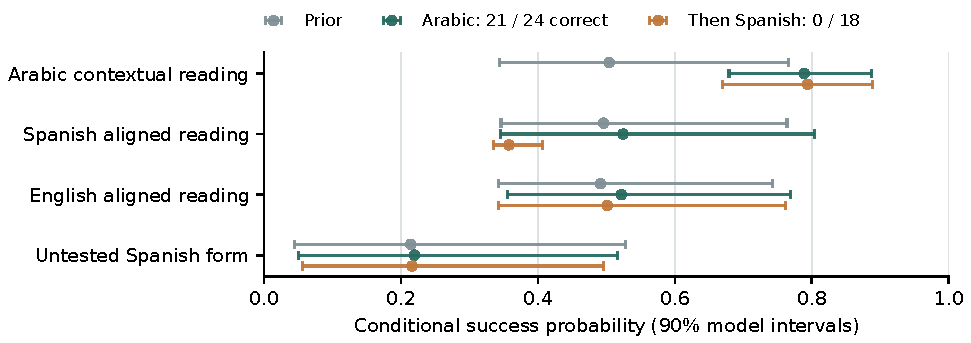
\includegraphics[width=.96\textwidth]{figures/learner_transfer.pdf}
\caption{Actual posterior predictions under three synthetic evidence
conditions. Points are means and horizontal lines are 90\% model intervals.
The Arabic responses inform a declared shared reading, while local lexical
effects and untested forms remain uncertain. Spanish counterevidence can
defeat the initial borrowed prediction. Differences among untouched
prior-only draws across independently seeded fits are Monte Carlo variation,
not learned foreign vocabulary.}
\label{fig:transfer}
\end{figure*}

The Arabic mean changes from \LearnerArabicPrior{} to
\LearnerArabicPosterior{}. The Spanish aligned-reading mean after Arabic
evidence is \LearnerSpanishBorrowed{}, with a broad interval; after its own
counterevidence it is \LearnerSpanishCounter{}. The unobserved Spanish
exceptional form remains prior-only, with mean \LearnerUntestedForm{}
after the Arabic evidence. Figure~\ref{fig:transfer} makes the distinction
between a shared reading and local word-form knowledge visible.

The Spanish all-failure condition is deliberately adverse. Because the
authored recognition task has a fixed guessing floor, its predicted success
cannot approach zero. This exposes a substantive likelihood assumption:
systematic mistakes and distractor preferences may require a different
response model. The experiment checks that local evidence is not erased by
pooling; it is not an estimate of negative transfer between human languages.

A separately generated sequence of 64 Bernoulli outcomes, with stipulated
success probability 0.85, has 59 successes under the fixed seed. On this one
sequence, the prior and updated Arabic predictions have Brier scores
\LearnerBrierPrior{} and \LearnerBrierPosterior{}, and log losses
\LearnerLogPrior{} and \LearnerLogPosterior{}. These proper scores describe
the supplied example. They do not establish superiority to knowledge tracing,
item-response models, or existing repetition systems, and they do not
constitute a cross-learner calibration study.

\subsection{Decision Arithmetic and a Fitted Example}

The decision module is tested against \LearnerExactCases{} hand-computable
finite-posterior cases. The basic case assigns equal probability to a root
gap and a pattern gap. Each corresponding support costs 0.2, and an ideal
diagnostic costs 0.1. Acting without information has risk 0.7; a diagnostic
followed by the appropriate support has risk 0.3. Information value is 0.5
and net improvement is 0.4. A noisy diagnostic with outcome probabilities
0.8 and 0.2 has information value 0.3 and net improvement 0.2.

\begin{figure*}[t]
\centering
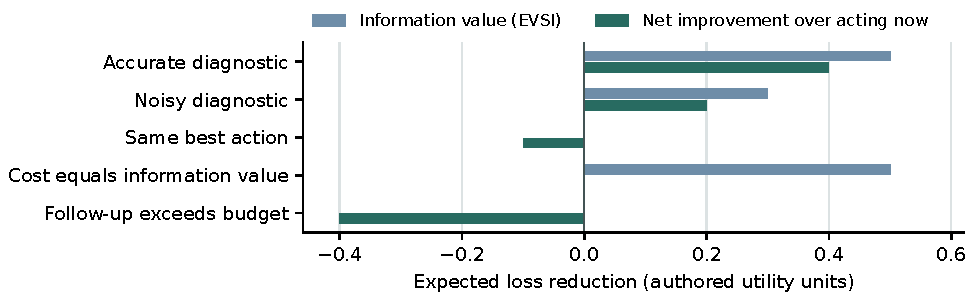
\includegraphics[width=.96\textwidth]{figures/learner_decisions.pdf}
\caption{Hand-computable cases evaluated by the shipped policy. Information
value is separated from net improvement after effort, delay, and remaining
budget. A question with an informative answer can have zero decision value
when the same support remains optimal. A positive information value can also
be insufficient to justify its cost. These are exact synthetic decision
checks, not measured learner benefits.}
\label{fig:decisions}
\end{figure*}

Other cases cover an uninformative question, an informative question whose
outcomes share the same best action, a known gap, break-even cost, a diagnostic
that consumes the follow-up support budget, and an explicit no-practice
constraint. All \LearnerExactCases{} cases pass. Additional tests preserve
covariance when multiple targets share joint posterior draws, reject
unsupported component bypasses, honor nonuniform weights, and fail safely
when a total computation bound is exceeded.

The report also sends a fitted posterior into the same policy.
Its synthetic history contains 20 successful Arabic base-recall responses
and 20 unsuccessful responses on a different lexical base with the relevant
Arabic pattern. The lowest-loss action supplies the authored pattern cue.
The full report retains its candidate losses and diagnostic outcome branches,
so this result can be inspected without inferring a diagnosis from the action
name alone.

\subsection{Temporal and Application Verification}

A separate dynamic fit predicts a lower success probability after 30 days
without an additional accepted opportunity. This checks the implemented
nonnegative decay term. It does not establish a measured forgetting curve.
Tests also cover disabled dynamics, mode separation, explicit cohort
authorization, task and parameter caps, deterministic replay, and
asynchronous cancellation.

The release's verification run includes \LearnerNodeTests{} passing
JavaScript unit tests, \LearnerDOMTests{} passing executable DOM/integration
tests, and \LearnerAPITests{} passing Python tests. The latter include the
actual new task's scorer and analysis references round-tripping through
FastAPI and SQLite. The application tests execute the shipping self-contained
HTML, select a goal, answer a task, recompute a posterior and decision, and
export the scoped calculation. They check that unrelated cards, schedules,
and reader content are preserved.

Cross-task exposure tests are particularly consequential. They verify
recognition-prompt to recall leakage, supplied-base to base-recall leakage,
an exceptional form shown under one task ID and answered under another,
same-form repetition, recorded component hints, future and expired exposures, and account/team
separation. The bridge independently reconciles these exposures for imported
events; it does not trust the UI alone. A response's own later feedback
cannot invalidate it retrospectively.

The full native-browser visual run was blocked because the execution
environment denied Chromium's socket creation. No claim is made here about
native-browser layout, real assistive technology, or native IndexedDB
durability. The DOM transaction fixture, actual server persistence tests,
source inspection, and compiled-bundle execution are distinct forms of
coverage, and the verification record states which were run.

\paragraph{Runtime.}
The saved numerical suite reports \LearnerRuntime{} milliseconds on its
recorded Node/Linux environment. This is a measured run of the bounded
synthetic cases, not a service-level guarantee or a benchmark on mobile
hardware. All candidate, observation, coefficient, sampling, and decision-work
limits are inspectable in source. Asynchronous fitting yields so the user can
continue or change context.

\section{Limits and Next Empirical Questions}

\paragraph{Linguistic and measurement validity.}
The 93 new tasks are a small authored slice. Richer morphology is bounded
to the declared Arabic, English, and Spanish examples; the remaining language
coverage consists of two vocabulary items in two response modes. All are
labelled authored and not independently instructor-reviewed. Dialect,
register, productive composition, phonological competence, valid alternative
answers, and task instruction comprehension require further work. Exact
answer matching measures the declared rubric, which can be narrower than
linguistic correctness.

\paragraph{Statistical limitations.}
The full decomposition is not generally identified by available responses.
Root, language, word, context, memory, and time effects can explain similar
patterns. Learned variances remain prior-sensitive, especially with few
groups. The shared-factor design expresses positive common variation, not an
arbitrary learned covariance or a causal transfer mechanism. Guessing,
lapses, difficulty offsets, and supported-component behavior are currently
authored settings. History truncation is reported and can change fitted
temporal covariates. Lightweight predictive diagnostics do not certify that
every latent quantity is well mixed.

\paragraph{Decision limitations.}
The implemented policy chooses one diagnostic followed by one terminal
action. Its loss concerns immediate completion, and its support model assumes
the declared cue supplies a component. That may be useful as an operational
assumption, but it requires empirical assessment. Long-horizon teaching,
retained learning, motivation, frustration, and opportunity costs beyond the
chosen task are not optimized. Observational practice trends are not
substituted for intervention effects. The user can always continue or choose
an optional task directly.

\paragraph{Evaluation needed for educational claims.}
A defensible human study would first review task content and rubrics, then
evaluate held-out task prediction with learner and item splits, compare
pooling structures and simpler baselines, inspect calibration by language and
response mode, and assess sensitivity to prior and nuisance settings.
Intervention claims require assignment or another justified causal design,
with delayed outcomes and interruption costs measured separately. The
present artifact makes those experiments implementable and auditable; their
results are not supplied by its graph or by successful software tests.

\section{Conclusion}

\Nabu{} 1.15.0 implements a concrete path from versioned task observations to
a hierarchical learner posterior and an actionable Bayesian decision.
Required ingredients, whole-form memory, explicit shared meanings, local
lexical forms, response modes, and time remain distinguishable in the model.
The decision calculation values information through its effect on available
actions. Its tests establish numerical and integration properties within
declared assumptions, while preserving the empirical questions that require
human evidence.

\bibliography{references}
\bibliographystyle{icml2026}
\clearpage
\appendix
\section{What Contrasts Can Identify in a Small Submodel}

It is helpful to distinguish a likelihood that becomes more informative from
one that identifies every latent mechanism. Consider a static, noise-free
submodel of one learner, one form, and one response mode. Let \(b\) be the
base-recall probability, \(p\) the pattern-execution probability, and \(r\)
the whole-form memory probability. Let the three tasks have exact population
response probabilities
\begin{equation}
 p_B=b,\qquad
 p_C=r+(1-r)p,\qquad
 p_F=r+(1-r)bp .
\end{equation}
Here \(B\) is base recall, \(C\) supplies the base and asks for the derived
form, and \(F\) supplies only the lexical action and form category.
If \(b\ne1\) and \(r\ne1\), the stipulated model permits
\begin{equation}
 r=\frac{p_F-bp_C}{1-b},\qquad
 p=\frac{p_C-r}{1-r}.
\end{equation}
This algebra explains why changing the tested ingredients can help.
It also exposes boundaries. When \(b\) is close to one, separating the memory
route from the pattern route is ill-conditioned. If all three response
probabilities are noisy estimates, the algebra need not yield admissible
probabilities without an appropriate likelihood. Different response modes
cannot be substituted for each other in these equations. A recognition
success is not an observation of \(p_B\) for production.

The full implemented model adds contextual, word, language, temporal, and
hierarchical variation; its generic diagnostic flags do not claim the above
three-equation identification result applies automatically. A different base
with the same bounded pattern supplies additional contrast while retaining
its own word memory and lexical knowledge.

\section{Why Inactive Coefficients Can Be Collapsed}

Partition the Gaussian effect vector into coefficients \(\theta_A\) that
appear in the accepted likelihood and coefficients \(\theta_U\) that do not.
Conditional on the variance groups, the declared prior factors over
coefficients. Therefore
\begin{equation}
\begin{split}
 p(\theta_A,\tau^2\mid D)
 &\propto p(D\mid\theta_A)\,
          p(\theta_A\mid\tau^2)\,p(\tau^2)\\
 &\quad\cdot\int p(\theta_U\mid\tau^2)\,d\theta_U\\
 &=p(D\mid\theta_A)\,
          p(\theta_A\mid\tau^2)\,p(\tau^2).
\end{split}
\end{equation}
The equality holds up to normalization. Sampling this marginal posterior
avoids adding many unobserved catalogue
effects to the variance-Gibbs transition. For a retained
\((\theta_A,\tau^2)\), drawing \(\theta_U\) from its conditional Gaussian
prior reconstructs a draw from the full posterior. The same reconstruction
is used across all task predictions for that draw; unrelated marginal
prediction arrays are never independently shuffled before computing EVSI.

The active set is defined by the accepted likelihood, not merely by a task
being present in the catalogue. Variance groups with no active coefficients
remain prior-only. Such labels distinguish a learned shared ability from a
group variance that has evidence elsewhere, and from a wholly untouched
prior. The export preserves all three cases.

\section{Reproduction and Artifact Layout}

The package retains the original graph, reader, account store, and backend.
The new pure modules separate tasks, audited input, posterior inference,
and decisions. The live UI writes through the existing content-event API.
No additional runtime package or external model provider is needed for
inference. Python and browser development dependencies are used only for
existing application hosting, testing, or paper generation.

\begin{table*}[h]
\caption{Implementation entry points and the contract each owns.}
\centering\small
\begin{tabular}{@{}p{.43\textwidth}p{.51\textwidth}@{}}
\toprule
Artifact & Responsibility \\
\midrule
\artifact{public/nabu-learner-tasks.js} &
Versioned task conditions, answer rules, component map, exposure identities,
source integrity gates. \\
\artifact{public/nabu-learner-observations.js} &
Actor-scoped evidence admission, conditioned tasks, exposure reconciliation,
bounded audit witnesses. \\
\artifact{public/nabu-learner-model.js} &
Hierarchical likelihood, collapsed sampling, prediction, hyperparameters,
diagnostics, explicit cohort API. \\
\artifact{public/nabu-learner-policy.js} &
Validated support effects, posterior loss, binary EVSI, budget and work bounds. \\
\artifact{public/nabu-learner-ui.js} &
Goal selection, live task delivery, idempotent writes, cancellation,
posterior refresh and export. \\
\artifact{tools/evaluate_learner.mjs} &
Independent reference calculation and seeded synthetic decision/prediction
report. \\
\artifact{docs/LEARNER_VERIFICATION.md} &
Recorded test outcomes and concrete limits of the execution environment. \\
\bottomrule
\end{tabular}
\end{table*}

Run the implementation and verification commands from the package root:
\begin{verbatim}
python start_local.py
npm test
python -m pytest -q
npm run test:learner
npm run evaluate:learner
python tools/build_standalone.py
\end{verbatim}
The DOM suites require the pinned jsdom development dependency, installed by
\texttt{npm install}; an existing installation can be selected with
\texttt{NABU\_TEST\_JSDOM}. The corresponding commands are
\texttt{npm run test:learner-ui} and the existing evidence, intent, and
next-step UI scripts. This test dependency is not shipped in the application's
runtime bundle.

Generate figures and the current paper from saved results:
{\footnotesize
\begin{verbatim}
python tools/build_learner_paper_figures.py
python tools/build_paper.py \
  --paper nabu-learner
\end{verbatim}
}
The figure manifest records the numerical report hash. The shipping HTML is
rebuilt with exact script and style hashes and a matching service-worker build
identity. The delivery manifest records file hashes for the release package
and paper. Earlier papers and baseline evaluation tools are preserved as
historical artifacts, not presented as results of this new learner model.

\section{Privacy and Practical Boundaries}

The current actor and selected team context delimit usable events. Separate
people are not pooled merely because their accounts belong to one team.
The cohort API is an explicit analytical facility whose caller must supply
authorized data and scope. A downloaded model record contains that actor's
scoped evidence and inferred posterior; it is an intentional user action,
not automatic telemetry.

The existing API accepts authenticated client observations. It does not
proctor performance or verify that a person answered unaided outside the
interface. Exact references and exposure controls make a record interpretable;
they cannot prevent all unrecorded help. The authored 30-minute exposure
window is a conservative operational rule, not an estimated forgetting time
or a claim that responses become statistically independent at its boundary.

Hint events are committed before displaying the cue. If the action is
cancelled while the save is pending, that event conservatively records
possibly supplied support even though the cue may never appear. This can
exclude a later response for the session. The present schema also lacks
the exact selected cue identity, so replay uses the union of maintained
possible cues for that task. Neither case is treated as proof of unaided
success.

\end{document}
